\newpage


\section{Wdrożenie wybranych metod detekcji}\label{sec:wdrozenie-metod-detekcji}

\subsection{Reverse Proxy --- Bot Blocker}\label{subsec:reverse-proxy-impl}

W infrastrukturze sklepu internetowego wdrożono serwer typu reverse proxy zlokalizowany przed backendem (zob. \autoref{fig:backend-reverse-proxy}).

\begin{figure}[H]
    \centering
    \captionsetup{width=.8\linewidth}
    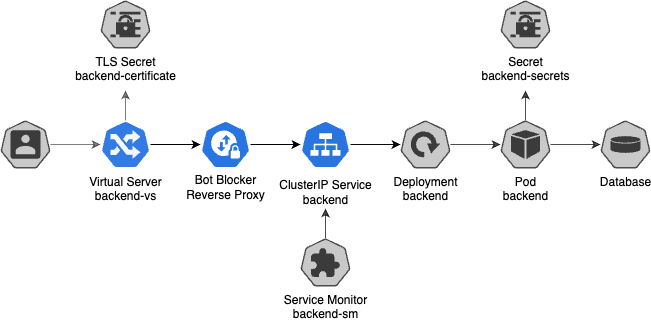
\includegraphics[width=\textwidth]{img/backend-reverse-proxy}
    \caption{Lokalizacja Reverse Proxy w infrastrukturze sklepu}
    \label{fig:backend-reverse-proxy}
\end{figure}

Serwer wykorzystuje oprogramowanie Nginx, które zostało rozszerzone o narzędzie Nginx Ultimate Bad Bot Blocker.
Zgodnie z opisem autorów, Ngnix Ultimate Bad Bot Blocker służące do obrony przed:
złośliwymi botami i złośliwymi agentami (\texttt{User-Agent}),
techniką Clickjacking, techniką Click Re-Directing,
Spam Referrer, Adware, Malware, Ransomware,
złośliwymi adresami IP z systemami anty-DDoS,
techniką wykrywania motywów Wordpress
oraz organizacjami SEO~\cite{nginx-ultimate-bad-bot-blocker}.

\autoref{lst:nginx-bot-blocker-conf} przedstawia konfigurację serwera.
Instrukcje \texttt{include} ładują konfiguracje dostarczane z Nginx Ultimate Bad Bot Blocker.
Serwer nasłuchuje na port 9090 i przekierowuje żądania na port 9000.
Żądania są przekazywane wraz z wszystkimi nagłówkami.
Dodatkowo, w celu monitoringu i zapewnienia audytowalności, włączono logowanie zdarzeń w niestandardowym formacie

Wdrożenie w środowisku Kubernetes wymagało konteneryzacji omawianego rozwiązania.
\autoref{lst:nginx-bot-blocker-dockerfile} przedstawia plik Dockerfile zawierający instrukcje budujące obraz \texttt{Bot Blocker Proxy}.
Jako bazę wykorzystano obraz \texttt{ngnix:stable}.
Instalacja Nginx Ultimate Bad Bot Blocker jest realizowana przez skrypt dostarczany przez twórców.

\begin{listing}[p]
    \begin{minted}[xleftmargin=10pt,linenos,breaklines]{nginx}
http {
    log_format  main  '$remote_addr - $remote_user [$time_local] "$request" '
                      '$status $body_bytes_sent "$http_referer" '
                      '"$http_user_agent" "$http_x_forwarded_for"';

    access_log  /var/log/nginx/access.log  main;

    include /etc/nginx/conf.d/botblocker-nginx-settings.conf;
    include /etc/nginx/conf.d/globalblacklist.conf;

    server {
	    listen  9090;
	    listen  [::]:9090;

	    include /etc/nginx/bots.d/ddos.conf;
        include /etc/nginx/bots.d/blockbots.conf;

	    location / {
		    proxy_pass                  http://localhost:9000;
		    proxy_pass_request_headers  on;
		    proxy_buffering             off;
	    }
    }
}
    \end{minted}
    \caption{Plik konfiguracyjny serwera reverse proxy}
    \label{lst:nginx-bot-blocker-conf}
\end{listing}

\begin{listing}[p]
    \begin{minted}[xleftmargin=10pt,linenos,breaklines]{docker}
FROM nginx:stable
RUN apt-get -y update && apt-get -y install wget
RUN wget https://raw.githubusercontent.com/mitchellkrogza/-
    nginx-ultimate-bad-bot-blocker/master/install-ngxblocker -O /usr/local/sbin/install-ngxblocker
RUN chmod +x /usr/local/sbin/install-ngxblocker
WORKDIR /usr/local/sbin
RUN ./install-ngxblocker -x
WORKDIR /
COPY nginx.conf /etc/nginx/
EXPOSE 9090
CMD ["nginx", "-g", "daemon off;"]
    \end{minted}
    \caption{Instrukcje budujące obraz reverse proxy}
    \label{lst:nginx-bot-blocker-dockerfile}
\end{listing}

\newpage

\subsection{Rate Limiting}\label{subsec:rate-limiting-impl}

Kolejnym wdrożonym zabezpieczeniem przed web scrapingiem był API Rate Limiting.
Wykorzystano możliwość uruchomionego wcześniej (zob. \autoref{subsubsec:ingress-controller}) Ngnix Ingress Controller
do tworzenia zasobów polityk (ang. \emph{Policy Resource}) dla zasobów typu \texttt{VirtualServer} i \texttt{VirtualServerRoute}.
Polityki te pozwalają na kontrolę dostępu (ang. \emph{access control}) i rate limiting~\cite{nginx-ingress-controller-policy-resource}.

Wdrożono politykę \emph{store-api-rate-limit-policy} ograniczającą liczbę żądań do 40 na minutę
dla jednego adresu IP (\texttt{binary\_remote\_addr}), z możliwością przekroczenia limitu o 5 (\texttt{burst}).
Pełną konfigurację \emph{store-api-rate-limit-policy} przedstawia \autoref{lst:rate-limiting-policy}.

Polityka została zaaplikowana do VirtualServer, który zarządza komunikacją z backendem (zob. \autoref{fig:backend-rate-limiting}).
Szczegółowa konfiguracja VirtualServer \texttt{backend-vs}, w tym wykorzystanie polityki \texttt{store-api-rate-limit-policy}, zostało przedstawione na \autoref{lst:rate-limiting-virtual-server}.
Widoczne tam sekcje \texttt{action.pass} mówią o tym, co ma się stać z ruchem pasującym do określonej ścieżki (\texttt{path}).
Rate limiting został zaaplikowany dla ścieżek z prefiksem \texttt{/store} (linia 18, \texttt{path: /store}), zatem dla Store API z pominięciem Admin API wykorzystywanym do zarządzania sklepem.


\begin{figure}[H]
    \centering
    \captionsetup{width=.8\linewidth}
    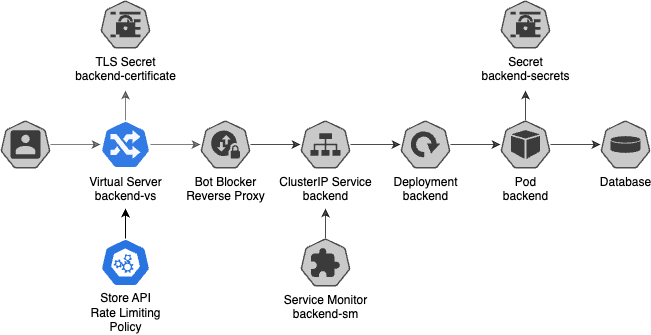
\includegraphics[width=\textwidth]{img/backend-rate-limiting}
    \caption{Polityka Rate Limiting w infrastrukturze sklepu}
    \label{fig:backend-rate-limiting}
\end{figure}

\begin{listing}[p]
    \begin{minted}[xleftmargin=10pt,linenos,breaklines]{yaml}
apiVersion: k8s.nginx.org/v1
kind: Policy
metadata:
  name: store-api-rate-limit-policy
  namespace: store
spec:
  rateLimit:
    rate: 40r/m
    key: ${binary_remote_addr}
    burst: 5
    zoneSize: 10M
    rejectCode: 429
    \end{minted}
    \caption{Manifest \texttt{store-api-rate-limit-policy}}
    \label{lst:rate-limiting-policy}
\end{listing}

\begin{listing}[p]
    \begin{minted}[xleftmargin=10pt,linenos,breaklines]{yaml}
apiVersion: k8s.nginx.org/v1
kind: VirtualServer
metadata:
  name: backend-vs
  namespace: store
spec:
  ingressClassName: public
  host: api.tulski.com
# tls: ...
  upstreams:
    - name: bot-blocker-proxy
      service: bot-blocker-proxy
      port: 9090
  routes:
    - path: /
      action:
        pass: bot-blocker-proxy
    - path: /store
      policies:
        - name: store-api-rate-limit-policy
      action:
        pass: bot-blocker-proxy
    \end{minted}
    \caption{Szczegółowa konfiguracja VirtualServer \texttt{backend-vs}}
    \label{lst:rate-limiting-virtual-server}
\end{listing}

\newpage

\subsection{Browser Fingerprinting}\label{subsec:browser-fingerprinting-impl}

Opracowano i wdrożono rozwiązanie korzystające z procesu browser fingerprintingu mające na celu identyfikację i blokowanie nieautoryzowanego dostępu do zasobów sklepu internetowego tulski przez scrapery.
Zasadę działania systemu przedstawia \autoref{fig:bot-detection-sequence}.

\begin{figure}[H]
    \centering
    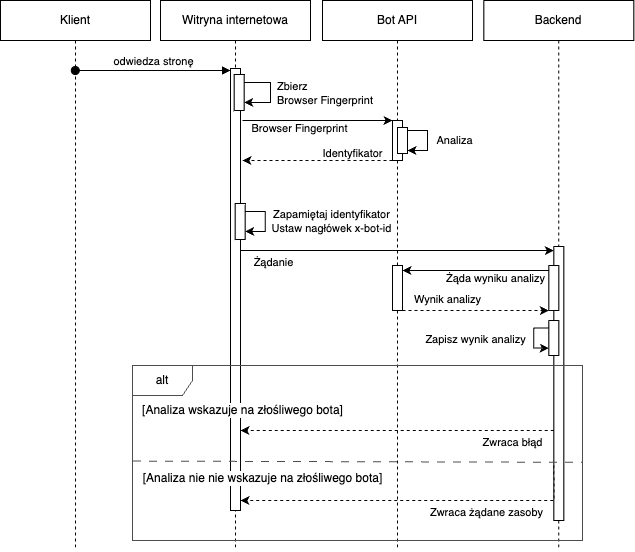
\includegraphics[width=.95\textwidth]{img/bot-detection-sequence}
    \caption{Diagram sekwencji rozwiązania wykorzystującego browser fingerprinting}
    \label{fig:bot-detection-sequence}
\end{figure}

Stworzono nową aplikację \texttt{Bot API} wraz z dedykowanym dla niej klientem \texttt{@tulski/\\bot-client}.
Dodatkowo, zmodyfikowano istniejącą witrynę internetową i backend.

\subsubsection{Bot API}

\texttt{Bot API} to aplikacja webowa napisana w języku TypeScript z wykorzystaniem platformy Express.js.
Środowiskiem uruchomieniowym aplikacji jest Node.js.
Do analizy odcisku przeglądarki wykorzystano bibliotekę \texttt{fpscanner}~\cite{github-fpscanner}.
Browser fingerprint jest poddawany 21 testom (zob. \autoref{lst:fpscanner-tests}), z których każdy
może zwrócić 3 wartości: \texttt{Consistent}, \texttt{Unsure} i \texttt{Inconsistent}.
Odcisk jest klasyfikowany jako pochodzący od złośliwego bota (\texttt{"bad\_bot"}) jeżeli:
\begin{itemize}
    \item więcej niż jeden test zwraca wartość \texttt{Inconsistent},
    \item przynajmniej jeden test zwraca wartość \texttt{Inconsistent} i przynajmniej jeden test zwraca wartość \texttt{Unsure}.
\end{itemize}

\begin{listing}[H]
    \begin{minted}[xleftmargin=10pt,linenos,breaklines]{text}
[
  "PHANTOM_UA", "PHANTOM_PROPERTIES", "PHANTOM_ETSL", "PHANTOM_LANGUAGE", "PHANTOM_WEBSOCKET", "MQ_SCREEN", "PHANTOM_OVERFLOW", "PHANTOM_WINDOW_HEIGHT", "HEADCHR_UA", "WEBDRIVER", "HEADCHR_CHROME_OBJ", "HEADCHR_PERMISSIONS", "HEADCHR_PLUGINS", "HEADCHR_IFRAME", "CHR_DEBUG_TOOLS", "SELENIUM_DRIVER", "CHR_BATTERY", "CHR_MEMORY", "TRANSPARENT_PIXEL", "SEQUENTUM", "VIDEO_CODECS"
]
    \end{minted}
    \caption{Tablica testów na obecność śladu złośliwego bota}
    \label{lst:fpscanner-tests}
\end{listing}


API udostępnia trzy końcówki.
\begin{enumerate}
    \item \texttt{GET /health} służący do monitorowania stanu aplikacji.\ Wykorzystywany przed Kubernetes w mechanizmie \texttt{Liveness Probe}.
    \item \texttt{POST /api/v1/analyze} przyjmujący na wejściu browser fingerprint, który jest poddawany analizie.
    Zwraca unikalny identyfikator przeprowadzonej analizy.
    \item \texttt{GET /api/v1/verify/:id} dający dostęp do wyniku analizy z wskazanym identyfikatorem (\texttt{id}).
    Zwraca obiekt JSON, który zawiera atrybut \texttt{result} przyjmujący wartość \texttt{"not\_detected"} lub \texttt{"bad\_bot"}.

\end{enumerate}
\noindent Aplikacja została wyposażona w podstawową walidację danych wejściowych.

\subsubsection{@tulski/bot-client}

\texttt{@tulski/bot-client} to biblioteka będąca dedykowanym klientem \texttt{Bot API}.
Biblioteka jest dostępna publicznie jako paczka w NPM Registry pod adresem: \url{https://www.npmjs.com/package/@tulski/bot-client}.
Jej Wykorzystanie polega na stworzeniu instancji klasy \texttt{BotClient}, a następnie wywołaniu metody \texttt{analyze()} zwracającej wynik analizy odcisku przeglądarki.
\texttt{@tulski/bot-client} zbiera browser fingerprint przy pomocy biblioteki \texttt{fp-collect}~\cite{github-fp-collect}.
Interfejs biblioteki przedstawia \autoref{lst:bot-client-types}.

\begin{listing}[H]
    \begin{minted}[xleftmargin=10pt,linenos,breaklines]{typescript}
export declare class BotClient {
    static load(baseUrl: string): Promise<BotClient>;
    constructor(baseUrl: string);
    analyze(): Promise<BotAnalysisResult>;
}
export interface BotAnalysisResult {
    id: string;
    created_at: Date;
    bot: "not_detected" | "bad_bot" | "good_bot";
}
    \end{minted}
    \caption{Definicja typów biblioteki \texttt{@tulski/bot-client}}
    \label{lst:bot-client-types}
\end{listing}

\subsubsection{Witryna internetowa}

W witrynie internetowej zaimplementowano \texttt{BotDetectionProvider}, wykorzystując powszechnie znany wśród specjalistów React wzorzec \texttt{Provider}.
\texttt{BotDetectionProvider} podczas wejścia na stronę:
\begin{enumerate}
    \item pobiera wynik analizy odcisku przeglądarki z lokalnego magazynu (ang. \emph{local storage}),
    \item dołącza identyfikator wyniku analizy jako nagłówek \texttt{x-bot-api} do żądań Store API\@.
\end{enumerate}
Gdy local storage nie zawiera wyniku analizy (na przykład przy pierwszym wejściu na stronę), \texttt{Provider} tworzy go wykorzystując bibliotekę \texttt{@tulski/bot-client} i zapisuje w magazynie.

\subsubsection{Backend}

Zmian wymagał również backend sklepu internetowego tulski.
Zaimplementowano interceptor działający dla końcówek \texttt{Store API}, który kolejno:
\begin{enumerate}
    \item weryfikuje obecność identyfikatora analizy odcisku palca w nagłówku \texttt{x-bot-api},
    \item pobiera ten identyfikator,
    \item komunikuję się z \texttt{Bot API} w celu pobrania pełnego wyniku analizy,
    \item weryfikuje czy odcisk przeglądarki wskazuje na złośliwego bota.
\end{enumerate}
W przypadku braku nagłówka \texttt{x-bot-api} w żądaniu, serwer zwróci błąd z kodem 403.
Jeśli analiza wykryje złośliwego bota, serwer odpowie kodem błędu 500.
